%
% strahlung.tex
%
% (c) 2025 Prof Dr Andreas Müller
%
% Minimalistisches 2D-TikZ-Diagramm eines Schwarzkörperstrahlers mit Kerze
\documentclass[tikz,border=5pt]{standalone}
\usetikzlibrary{patterns,shapes.misc}

\begin{document}
	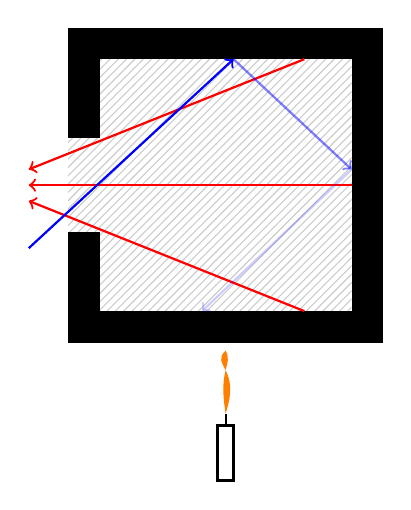
\begin{tikzpicture}
		% Parameter für Würfel
		\def\s{4}         % Seitenlänge des Blocks
		\def\t{0.4}       % Wandstärke
		\def\ah{1.2}      % Höhe der Apertur (Loch)
		\pgfmathsetmacro{\acy}{2}                      % y-Koordinate des Lochzentrums
		\pgfmathsetmacro{\abot}{\acy - \ah/2}        % unteres Ende der Apertur
		\pgfmathsetmacro{\atop}{\acy + \ah/2}        % oberes Ende der Apertur
		
		% Innenraum (schraffiert)
		\fill[pattern=north east lines, pattern color=black!20]
		(0,\t) rectangle (\s-\t,\s-\t);
		
		% Außenwände (dick, schwarz)
		\fill[black] (0,0) rectangle (\s,\t);           % Boden
		\fill[black] (0,\s-\t) rectangle (\s,\s);     % Decke
		\fill[black] (\s-\t,0) rectangle (\s,\s);     % rechte Wand
		\fill[black] (0,0) rectangle (\t,\abot);        % linke Wand unten
		\fill[black] (0,\atop) rectangle (\t,\s);      % linke Wand oben
		
		% Rote Pfeile, die von innen durch das Loch nach außen
		\draw[->, thick, red] (\s-\t,\acy) -- (-0.5,\acy);
		\draw[->, thick, red] (3,\t) -- (-0.5,{\acy-0.2});
		\draw[->, thick, red] (3,{\s-\t}) -- (-0.5,{\acy+0.2});
		
		% Kerze unter dem Block
		\pgfmathsetmacro{\flametip}{\t-0.5}                  % Flammenspitze an Blockunterkante
		\pgfmathsetmacro{\flameheight}{0.8}              % Höhe der Flamme
		\pgfmathsetmacro{\flamebase}{\flametip - \flameheight} % Flammenboden
		\pgfmathsetmacro{\wicklength}{0.15}              % Dochtlänge
		\pgfmathsetmacro{\wickbottom}{\flamebase - \wicklength} % Docht unten
		
		% Kerzenkörper und Flamme
		\fill[white] (1.9,{\wickbottom - 0.7}) rectangle (2.1,{\wickbottom});
		\draw[line width=1pt] (1.9,{\wickbottom - 0.7}) rectangle (2.1,{\wickbottom});
		\draw[line width=0.8pt] (2.0,{\wickbottom}) -- (2.0,{\flamebase});
		\fill[orange]
		(2.0,{\flamebase}) .. controls (2.2,{\flamebase + 0.6}) and (1.8,{\flamebase + 0.6}) ..
		(2.0,{\flametip}) .. controls (2.1,{\flamebase + 0.6}) and (1.9,{\flamebase + 0.6}) .. cycle;
		
		% Blauer Pfeil von außen ins Innere mit Reflexionen und abnehmender Opazität
		% Erstes Eindringen
		\draw[->, thick, blue, opacity=1]
		(\t-0.9,\acy - 0.8) -- ({\s-\t-1.5},{\s-\t});
		% erste Reflexion
		\draw[->, thick, blue, opacity=0.5]
		({\s-\t-1.5},{\s-\t}) -- (3.6,\t+1.8);
		% zweite Reflexion
		\draw[->, thick, blue, opacity=0.2]
		(3.6,\t+1.8) -- (1.7,\t);
		
	\end{tikzpicture}
\end{document}
